
\documentclass[xcolor={dvipsnames,table}]{beamer}
\usepackage{tikz}
\usepackage{wasysym}
\usepackage{color}
\usepackage{graphicx}
\usepackage{listings}
\usepackage[T2A]{fontenc}
\usepackage[russian,english]{babel}
\usepackage[utf8]{inputenc}
\date{\today}
\lstdefinestyle{basic}{
    captionpos=t,%
    basicstyle=\footnotesize\ttfamily,%
    numberstyle=\tiny,%
    numbers=left,%
    stepnumber=1,%
    frame=single,%
    showspaces=false,%
    showstringspaces=false,%
    showtabs=false,%
    %
    keywordstyle=\color{blue},%
    identifierstyle=,%
    commentstyle=\color{gray},%
    stringstyle=\color{magenta}%
}
\usetheme{Madrid}
\usetikzlibrary{shadows}
\title[]{Исследование возможностей сервера OpenLDAP для аутентификации пользователей СУБД PostgreSQL}
\date{27 января 2014}
\author{Воронин Д.Л., Муравьёв С.К.}

\begin{document}


\frame{\titlepage}


\defverbatim[colored]\hgdlnpfppbplcjckcinkgamfnelbbbdg{
\begin{lstlisting}[style=basic, xleftmargin=1.5em, xrightmargin=1em, numbers=none]
hostssl all all 192.168.100.0/24 ldap 
ldapserver=192.168.100.3 
ldapprefix="uid=" 
ldapsuffix=",ou=People,dc=ldap-server,dc=ru"
\end{lstlisting}
}
\defverbatim[colored]\nmdchefddejglkmppkcaagoogamgajgm{
\begin{lstlisting}[style=basic, xleftmargin=1.5em, xrightmargin=1em, numbers=none]
dn: uid=nivanov,ou=People,dc=ldap-server,dc=ru
uid: nivanov
cn: Nikolay Ivanov
objectClass: account
objectClass: posixAccount
objectClass: top
objectClass: shadowAccount
userPassword: {SSHA}US0VGNxhxro/QD3B4wIbjRa5re9i8cX1
shadowLastChange:15997
shadowMin:0
shadowMax:99999
shadowWarning: 7
loginShell: /bin/bash
uidNumber: 501
gidNumber: 501
homeDirectory: /home/nivanov
\end{lstlisting}
}


\begin{frame}
 \frametitle{Обзор основных методов аутентификации СУБД PostgreSQL}
  


\begin{itemize}
  \item <1-6>Trust
  \item <2-6>Password
  \item <3-6>Ident
  \item <4-6>Peer
  \item <5-6>PAM
  \item <6>LDAP
\end{itemize}

  
\end{frame}
\begin{frame}
 \frametitle{Схема работы метода PAM}
  


\begin{center}
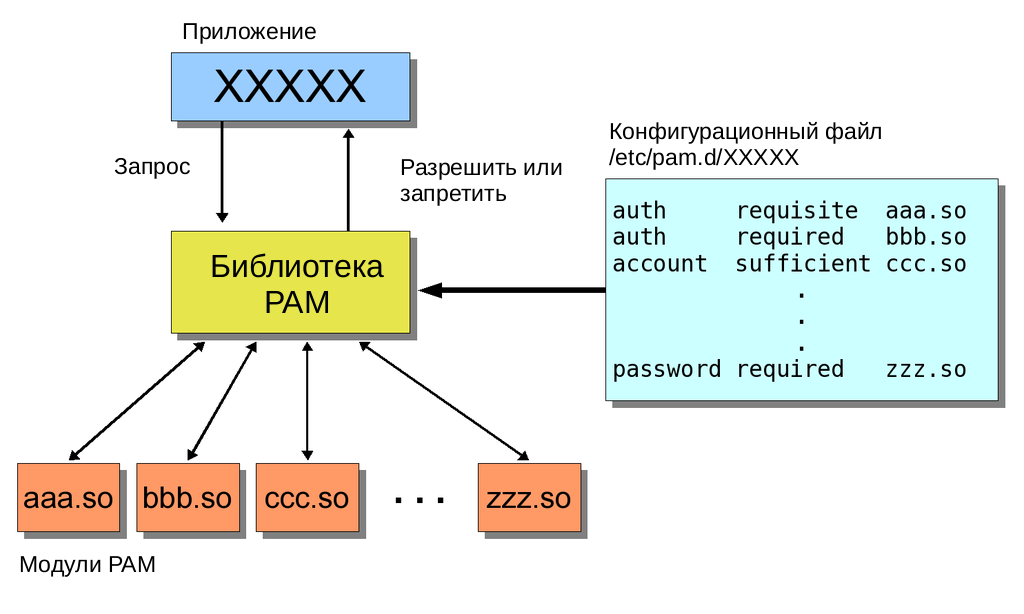
\includegraphics[ height=0.75\textheight]{files/pam.png}
\end{center}

  
\end{frame}
\begin{frame}
 \frametitle{Информационное дерево каталога LDAP}
  


\begin{center}
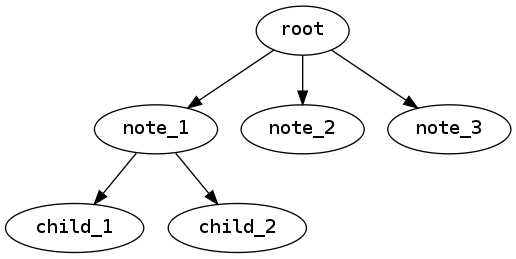
\includegraphics[ height=0.65\textheight]{files/DIT.png}
\end{center}

  
\end{frame}
\begin{frame}
 \frametitle{Схема работы стенда}
  

\begin{center}
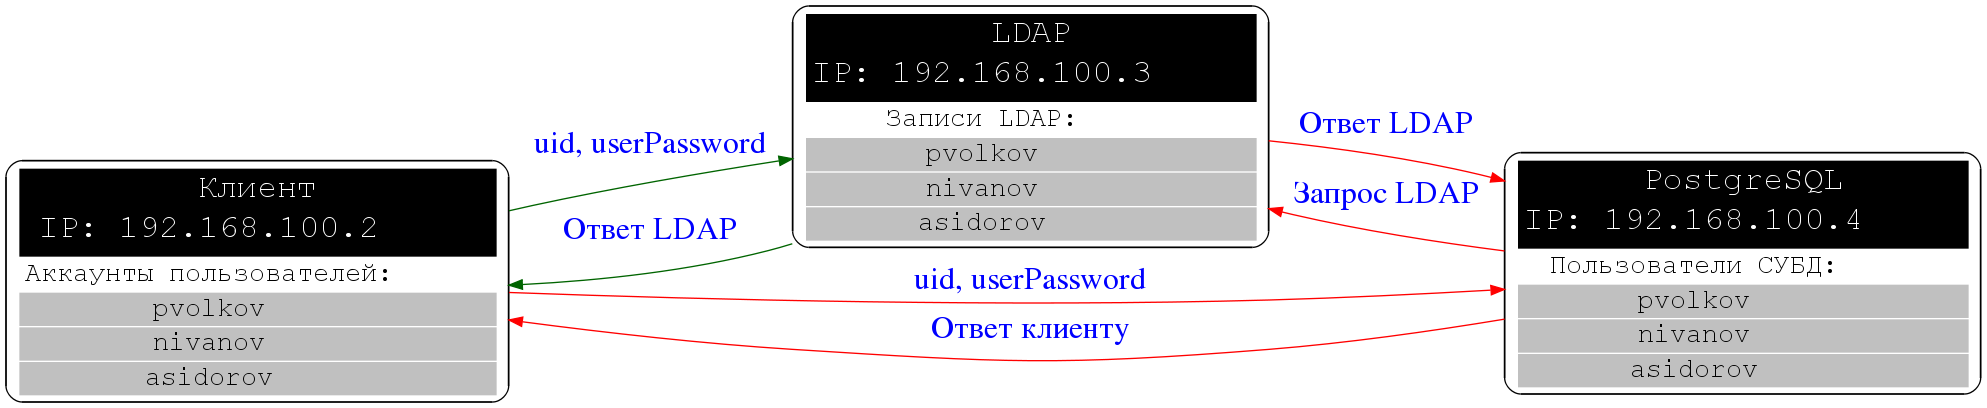
\includegraphics[ height=0.75\textheight]{files/cluster.png}
\end{center}

  
\end{frame}
\begin{frame}
 \frametitle{Запись аккаунта пользователя LDAP}
  


\nmdchefddejglkmppkcaagoogamgajgm



  
\end{frame}
\begin{frame}
 \frametitle{Аутентификация пользователя на клиентской машине}
  


\begin{center}
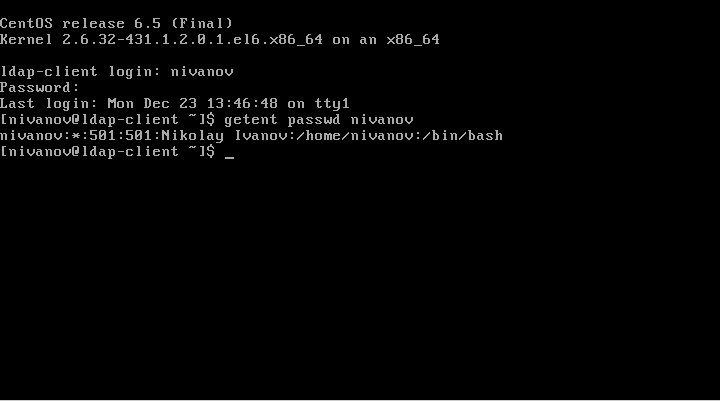
\includegraphics[ height=0.70\textheight]{files/getent.png}
\end{center}

  
\end{frame}
\begin{frame}
 \frametitle{Соединение клиента с сервером LDAP}
  

\begin{center}
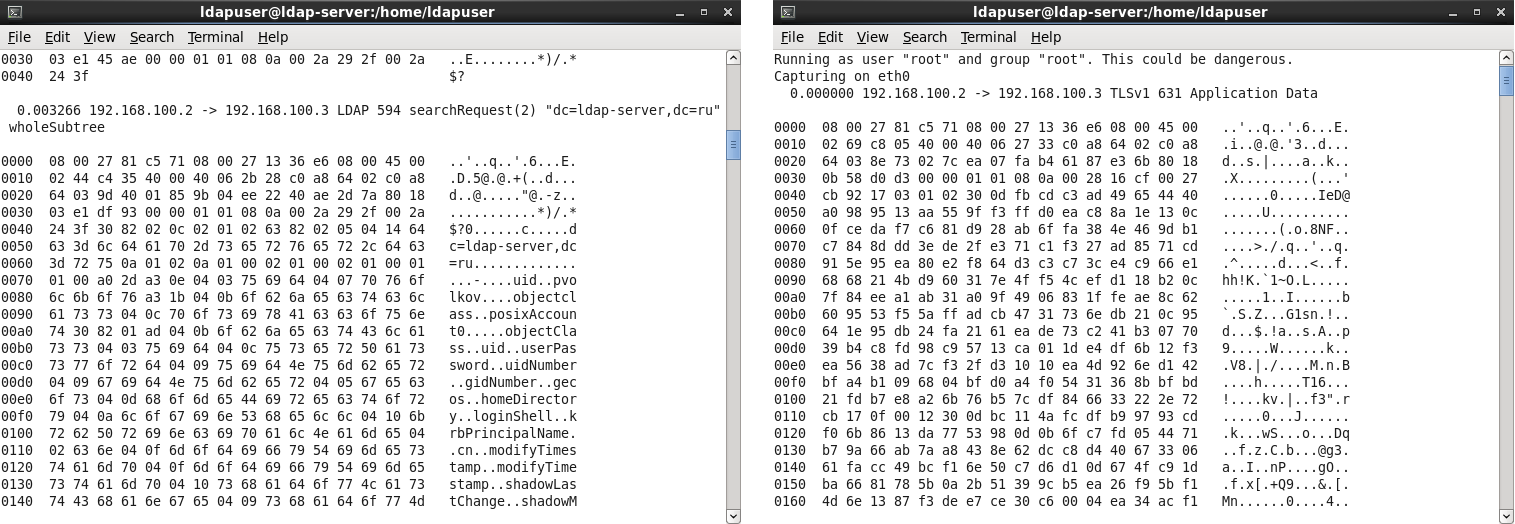
\includegraphics[ height=0.45\textheight]{files/ldap+ldaps.png}
\end{center}

\vspace{ 1em }

Слева представлен вывод утилиты \texttt{tethreal} для соединение клиента и сервера LDAP по протоколу \texttt{ldap}, справа --- по протоколу \texttt{ldaps} (\emph{LDAP security})

  
\end{frame}
\begin{frame}
 \frametitle{Аутентификация клиентов СУБД PostgreSQL по методу LDAP}
  


В файл \texttt{/var/lib/pgsql/9.3/data/pg\_hba.conf} требуется добавить строку:

\vspace{ 1em }



\hgdlnpfppbplcjckcinkgamfnelbbbdg



  
\end{frame}
\begin{frame}
 \frametitle{Достигнутые результаты}
  

\begin{itemize}
  \item Произведено исследование основных методов аутентфиикации СУБД PostgreSQL. Выявлены их достоинства и недостатки.
  \item Исследованы возможности сервера OpenLDAP.
  \item Описан процесс настройки метода аутентификации LDAP в PostgreSQL.
\end{itemize}

  
\end{frame}


\end{document}

